\section{Appendix}
\subsection{Observe the impact of scheduled positive events: students' stress during exam intervals in two situations}
To further observe the influence of uplift events for students facing stressor events,
we statistic all the stressful intervals~\cite{Li2017Analyzing} detected surround the scheduled examinations over the 124 students during their high school career.
For each student, we divide all his/her stressful intervals into two sets:
1) stressful intervals under the influence of neighbouring uplift events (e.g., \emph{Halloween activity}), and 2) independent stressful intervals.
Figure~\ref{fig:frequency} shows five measures of each student during the above two conditions:
the \emph{accumulated stress}, the \emph{average stress} (per day), the \emph{length of stressful intervals},
the \emph{frequency of academic topic words}, and the \emph{ratio of academic stress among all types of stress}.
For each measure, we calculate the average value over all eligible slides for each student.
\begin{figure}
\centering
\caption{Compare students' stress during exam intervals in two situations:
1) affected by neighboring uplift events (U-SI), 2) no uplift events occurred nearby (SI)}
\includegraphics[width=\linewidth]{figs/frequency.eps}
\label{fig:frequency}
\end{figure}

\subsection{Algorithm 1: Select candidate intervals impacted by positive events}
\label{alg:alg1}
Let the sub-series $w_{<a,b>} = [s^{'}_a, \cdots, s^{'}_b]$ as a \emph{wave},
where $s^{'}_v$ $= {vally(w_{<a,b>})}$ is the minimum stress value,
$s^{'}_p$ $= peak(w_{<a,b>})$ is the maximal stress value during $\{s^{'}_a,\cdots,s^{'}_b\}$,
and $s^{'}_a \leq s^{'}_{a+1} \leq \cdots \leq s^{'}_p \leq s^{'}_{p+1} \leq \cdots \leq s^{'}_b$.

\begin{table*}
\begin{center}
\caption{\small{Algorithm 1: Select candidate stress intervals impacted by positive events.}}
\begin{tabular}{l} \hline
A candidate interval $I = <w_1,\cdots, w_i,\cdots, w_m>$ is identified with following rules:\\
\textcircled{1} $s^{'}_1 = 0$, $s^{'}_m = 0$. $\forall s^{'}_j \in \{s^{'}_2,\cdots,s^{'}_{m-1}\}$, $s^{'}_j > 0$.\\
\textcircled{2} Let $w_i$ be the biggest wave in current candidate interval, with $peak(w_i) = \omega$, $\forall $ wave $w_j \in I$, $peak(w_j)<=peak(w_i)$.\\
\textcircled{3} For $w_k$ before the interval biggest wave $w_i$ , i.e., $\forall w_k \in <w_1,\cdots,w_{i-1}>$, $peak(w_{k+1})>=peak(w_k)$, $vally(w_{k+1}) >= peak(w_k)$.\\
\textcircled{4} For $w_k$ behind the interval biggest wave $w_i$, i.e.,  $w_k \in <w_{i}, \cdots, w_m>$, $peak(w_{k+1})<=peak(w_k)$, $vally(w_{k+1}) <= peak(w_k)$.\\\hline
\end{tabular}
\end{center}
\end{table*}

\subsection{Algorithm2: Identify stressful intervals impacted by positive events.}
\label{alg:alg2}
For each candidate interval,
a Poisson based probability model~\cite{Li2017Analyzing} is adopted to measure how confidently the current interval is a stressful interval.
Here a teen's stressful posting rate under stress ($\lambda_1$) and normal conditions ($\lambda_0$) are modeled as two independent poisson process:
\begin{equation}
Pr[N=n|\lambda_i]=\frac{e^{-\lambda_i T}{(\lambda_i T)}^n}{n!}
\end{equation}
where $i\in\{0,1\}$, $n=0,1,\cdots,\infty$.
We expect that $\lambda_1 > \lambda_0$, and measure the probability as $P(\lambda_1>\lambda_0|N_1, T_1, N_0, T_0)$,
where $N_1, N_0$ are the number of stressful posts, and $T_1, T_0$ are time duration corresponding to $\lambda_1$ and $\lambda_0$.
Without loss of generality, we assume a Jeffreys non-informative prior on $\lambda_1$ and $\lambda_0$,
and infer the posterior distribution $P(\lambda_1|N_1)$ and $P(\lambda_0|N_0)$ according to Bayes Rule.
Thus for current interval $I_1$ and historical normal interval $I_0$,
the quantified probability $\beta = P(\lambda_1>\lambda_0|I_1,I_0)$ $\in (0,1)$ indicates the confidence whether $I_1$ is a stressful interval.


\subsection{Algorithm3: judge stressful intervals into SI or U-SI}
\label{alg:alg3}
In this part, we filter out two sets of stressful intervals: stressful intervals without the impact of uplift events (SI),
and stressful intervals under the impact of uplift events (U-SI).
For a detected stressful interval $I = <t_1,\cdots,t_n>$, we consider the temporal order between $I$ and any detected uplift event $u$ happened at time point $t_u$:
\begin{itemize}
\item If the uplift event $u$ happens during the stressful interval, i.e., $t_u \in [t_1,t_n]$, the uplift interval $I$ is judged as $I \in SI$.
\item For the uplift event happening nearby a stressful interval,
we also consider the probability that it conducts impact on the teen's stressful interval.
Here the gap between $t_u$ and $I$ is limited to $\xi$, i.e.,
if $t_u \in [t_{1}-\xi, t_1)\cup(t_{n},t_{n}+\xi]$, then $I \in SI$.
%The setting of parameter $\xi$ is discussed in experiment section.
\end{itemize}
If a stressful interval satisfies none of the above conditions, we classify it into the U-SI set.

\subsection{Model 1: quantify significant restoring impact conducted by uplift events}
\label{mod:mod1}
For each teen, three groups of behavioral measures are considered: \emph{posting behavior},
\emph{stress intensity} and \emph{linguistic expressions},
indicated as \bm{${<D_p}$},\bm{${D_s}$},\bm{${D_l>}$}, respectively.
To measure the correlation for each group of positive and stressful behavioral measures,
the Euclidean distance is adopted to calculate the distance of structured points in $A_1$ and $A_2$.

For each point $\ell x \in A=A_1\bigcup A_2$,
let $NN_r(\ell_x,A)$ be the function to find the $r-$th nearest neighbor of $\ell_x$.
Specifically, according to the three group of measures,
three sub-functions of $NN_r(.)$ are defined as $PNN_r(.)$, $SNN_r(.)$ and $LNN_r(.)$,
corresponding to the teen's posting behaviors, stress intensity and linguistic expressions in each stressful interval,  respectively.

For point $\ell_x$ with posting behavior matrix \bm{${D_p^x}$}, stress intensity matrix \bm{${D_s^x}$},
and linguistic expression matrix \bm{${D_l^x}$},
the $r$-th nearest neighbor of $\ell_x$ in each measure is denoted as:
\begin{equation}
\begin{aligned}
& PNN_r(\ell_x,A)
= \{y | min\{||\textbf{D}_p^x-\textbf{D}_p^y ||_2\}, y\in(A/\ell_x)\} &\\
& SNN_r(\ell_x,A)
= \{z | min\{||\textbf{D}_s^x-\textbf{D}_s^z ||_2\}, z\in(A/\ell_x)\} \\
& LNN_r(\ell_x,A)
= \{w | min\{||\textbf{D}_l^x-\textbf{D}_l^w ||_2\}, w\in(A/\ell_x)\} &
 \end{aligned}
 \end{equation}
The $r$-th nearest neighbor considering all three groups of measures is denoted as:
\begin{align}
&NN_r(\ell_x,A) = \{v | min\{a \times ||\textbf{D}_p^x-\textbf{D}_p^v||_2+\\
&b \times ||\textbf{D}_s^x-\textbf{D}_s^v||_2+
c \times ||\textbf{D}_l^x-\textbf{D}_l^v||_2\}, v\in(A/\ell_x) \}
\end{align}
In this study, we set $a = b = c = 1/3$.
Next, let $I_r(\ell_x,A1,A2)$ be the function denoting whether the $r$-th nearest neighbor is in the same set with $\ell_x$:
\begin{equation}
I_r(\ell_x,A_1,A_2) =
\left\{ \begin{array}{ll}
1, \quad if \ell_x \in A_i  \&\& NN_r(\ell_x,A)\in A_i,\\
0, \quad otherwise
\end{array}
\right.
\end{equation}
Let $T_{r,n}$ denote the proportion that pairs containing two points from the same set among all pairs formed by $\ell_x \in A$
and its $k$ nearest neighbors:
\begin{equation}
T_{k,n}= \frac{1}{n\times k}\sum_{i=1}^{n}\sum_{j=1}^{k}I_j(x,A_1,A_2)
\end{equation}
The value of $T_{k,n}$ shows how differently the points in the two testing sets (SI and U-SI) perform in three groups of measures.
If the value of $T_{r,n}$ is close to $1$,
it can be shown that the two underlying distributions $F^{(1)}$ and $F^{(2)}$ for $SI$ and U-SI are significantly different,
indicating current uplift events conduct obvious restoring impact on the teens' stress series.
Let $\lambda_1=|A_1|$ and $\lambda_2=|A_2|$, the statistic value $Z$ is denoted as:
\begin{align}
&Z=(nr)^{1/2}(T_{r,n}-\mu_{r})/\sigma_{r}\\
&\mu_r=(\lambda_1)^2+(\lambda_2)^2\\
&{\sigma_r}^2=\lambda_1\lambda_2+4{\lambda_1}^2{\lambda_2}^2
\end{align}
where $\mu_r$ is the expectation and ${\sigma_r}^2$ is the variance of $Z$.
Based on hypothesis test theory \cite{Johnson2012Applied},
when the size of the testing set ($\lambda_1$ and $\lambda_2$) are large enough,
$Z$ obeys a standard Gaussian distribution.

Thus we judge whether the uplift events have conducted significant restoring impact on the teen's stress series as follows:
if $f(SI,USI)=(nr)^{1/2}(T_{r,n}-\mu_{r})/{\mu_r}^2>\alpha$ ($\alpha = 1.96$ for $P=0.025$),
then the hypothesis $H_1$ is true.

